\documentclass[arbeit=master,oneside,BCOR=12mm]{ArbeitRST}
% Die Option BCOR legt den Rand für die Bindekorrektur links fest
% (verschiebt das ganze Dokument nach rechts auf dem Papier, damit
% Platz zum Binden ist


% Paket zum Erzeugen von Blindtext 
% ================================
% (ist nur für dieses Beispieldokument sinnvoll)
\usepackage{blindtext}


% Zwei Parameter zum Verändern des Layouts
% ========================================
% \parindent -> Legt fest, mit welcher Einrückung jeder neue
%               Absatz beginnen soll
% \parskip -> Legt fest, wieviel vertikaler Abstand zwischen zwei
%             Absätzen liegen soll
%
% Tipp: Entweder parindent auf Null und parskip auf einen Wert
% ungleich Null (z.B. 2ex) oder umgekehrt. Beide Werte ungleich
% Null macht satztechnisch keinen Sinn. 1ex = Breite des 
% Buchstabens x
\setlength{\parindent}{0ex}
\setlength{\parskip}{2ex}


% Einige Einstellungen für das hyperref-Paket
% =========================================== 
% Hiermit können Links, Gleichungsnummern etc. farbig dargestellt
% werden was die Navigation im elektronischen Dokument vereinfacht. An
% dieser Stelle können Sie die Farbgebung anpassen. Druckversion bitte
% ohne farbige Links erstellen, siehe Option unten!
\hypersetup{
    unicode=false,          % non-Latin characters in Acrobat’s bookmarks
    pdftoolbar=true,        % show Acrobat’s toolbar?
    pdfmenubar=true,        % show Acrobat’s menu?
    pdffitwindow=false,     % window fit to page when opened
    pdfstartview={FitH},    % fits the width of the page to the window
    pdftitle={RST Vorlage}, % title
    pdfauthor={Author},     % author
    pdfsubject={Subject},   % subject of the document
    pdfcreator={Creator},   % creator of the document
    pdfproducer={Producer}, % producer of the document
    pdfkeywords={keyword1} {key2} {key3}, % list of keywords
    pdfnewwindow=true,      % links in new window
    colorlinks=true,        % false: boxed links; true: colored links
    linkcolor=blue,         % color of internal links (change box color with linkbordercolor)
    citecolor=green,        % color of links to bibliography
    filecolor=magenta,      % color of file links
    urlcolor=cyan           % color of external links
}

% Entfernt die farbigen Markierungen - bitte Druckversion mit dieser Option kompilieren
%\hypersetup{hidelinks}



% =================================================================
\begin{document}

% Titelseite
% ==========

% Name des Verfassers
\author{Martin P. Mustermann}

% Geburtsort
\geburtsort{Dresden}

% Geburtsdatum
\geburtsdatum{1. Januar 1912}

% Titel der Arbeit
\title{Über den Einfluss hochfrequenter mechanischer Oszillationen auf das Schaltverhalten supraleitender PID-Regler auf Quantenbasis}

% Untertitel
\subtitle{Eine Fallstudie unter besonderer Berücksichtigung stochastischer Einflüsse}

% Angabe der Betreuer
\betreuer{Betreuer 1}
\betreuer{Betreuer 2}

% Datum der Einreichung
\date{2. Februar 2222}

% Titelseite erstellen
\maketitle


% Selbstständigkeitserklärung
% ===========================

% Ort der Selbstständigkeitserklärung (Standard: Dresden)
\selbstort{Pirna}

% Datum der Selbstständigkeitserklärung (Standard: aktuelles Systemdatum)
\selbstdatum{1. Januar 2016}

% Selbstständigkeitserklärung erstellen
\selbststaendigkeitserklaerung


% Kurzfassung / Abstract
% ======================
\kurzfassung{An dieser Stelle fügen Sie bitte eine deutsche Kurzfassung ein.}{Please insert the English abstract here.}


% Inhaltsverzeichnis
% ==================
\tableofcontents


% Inhalt kann entweder in separate LaTeX-Dateien ausgelagert werden (hier: inhalt.tex)
% und dann mittels \input{} geladen werden...
\chapter{Erläuterungen zur Klasse ArbeitRST}
In den folgenden Abschnitten werden einige Erläuterungen zur \LaTeX-Dokumentenklasse \texttt{ArbeitRST.cls} gegeben werden. Diese basiert auf der Klasse \texttt{scrbook} aus dem KOMA-Script-Paket und kann daher mit Hilfe der Methoden aus diesem Paket modifiziert werden. Für nähere Informationen dazu sei auf die KOMA-Script-Anleitung\footnote{Diese kann unter der URL \url{http://www.ctan.org/pkg/koma-script} heruntergeladen werden.} und die Website
\begin{center}
	\url{http://www.komascript.de/}
\end{center}
verwiesen. 

Die wesentlichsten Änderungen gegenüber der ursprünglichen Klasse bestehen in einer angepassten Titelseite und der hinzugefügten Selbstständigkeitserklärung.



% ====================================================
\section{Informationen zu schriftlichen Arbeiten am RST}
Informieren Sie sich in der für Sie relevanten Prüfungsordnung über die \emph{Anzahl der geforderten Exemplare} die eingereicht werden müssen. Bitte beachten Sie, dass jedes dieser Exemplar die \emph{Aufgabenstellung} enthalten muss. Lassen Sie diese bitte beim Binden zwischen der Titelseite und der Selbstständigkeitserklärung einfügen. Eines der Exemplare muss dabei das \emph{originale}, vom Vorsitzenden des Prüfungsausschusses und dem verantwortlichen Hochschullehrer unterzeichnete, Dokument enthalten, bei den restlichen genügen Kopien. Bitte beachten Sie, dass die Arbeit \emph{einseitig} ausgedruckt werden muss. Ausschlaggebend für die fristgemäße Einreichung ist die \emph{Bestätigung des Prüfungsamtes}. Informieren Sie sich daher im \emph{Vorfeld} über die Öffnungszeiten am Abgabetag. Sollte das Prüfungsamt geschlossen haben, ist es in der Regel möglich mit den Mitarbeitern eine individuelle Vereinbarung zu treffen.


% ====================================================
\section{Die Titelseite}
Die Titelseite kann über die in Tabelle \ref{tab:titel} angegebenen Befehle angepasst werden.
\begin{table}[htbp]
\caption{Befehle zum Anpassen der Titelseite}
\label{tab:titel}
\begin{tabular}{lp{12cm}}
Befehl & Bedeutung\\
\toprule
\verb|\author| & legt den Namen des Autors der Arbeit fest\\
\verb|\geburtsdatum| & legt das Geburtsdatum des Autors fest\\
\verb|\geburtsort| & legt das Geburtsort des Autors fest\\
\verb|\title| & legt den Titel der Arbeit fest\\
\verb|\subtitle| & legt den Untertitel der Arbeit fest\\
\verb|\betreuer| & fügt einen Betreuer hinzu\\
\verb|\date| & legt das Einreichungsdatum der Arbeit fest -- \newline wird dieser Befehl nicht aufgerufen wird standardmäßig das zum Kompilationszeitpunkt eingestellte Systemdatum verwendet.\\
\bottomrule
\end{tabular}
\end{table}



% ====================================================
\section{Die Selbstständigkeitserklärung}
In der Selbstständigkeitserklärung werden automatisch der Typ der Arbeit, ihr Titel sowie der Name des Autors übernommen. Der Ort kann über den Befehl \verb|\selbstort| geändert werden, wobei standardmäßig "`Dresden"' verwendet wird. Das Datum ist standardmäßig identisch zum Einreichungsdatum, kann aber mit dem Befehl \verb|\selbstdatum| geändert werden.



% ====================================================
\section{Kurzfassung}
Eine Kurzfassung der Arbeit kann mit dem Befehl \verb|\kurzfassung{deutsch}{englisch}| eingefügt werden. Das erste Argument entspricht dabei der deutschen, das zweite der englischen Version.



% ====================================================
\section{Auswahl des Typs der Arbeit}
Zur Auswahl des Typs der Arbeit steht die Klassenoption \texttt{arbeit} zur Verfügung. Mit dieser können sie zwischen Diplom-, Master- und Studienarbeit sowie dem Bericht zum Forschungspraktikum auswählen:
\begin{table}[hbtp]%
\caption{Auswahl des Typs der Arbeit mittels Klassenoptionen}
\centering
\begin{tabular}{cc}
Diplomarbeit & \verb|\documentclass[arbeit=diplom]{ArbeitRST}|\\
Masterarbeit & \verb|\documentclass[arbeit=master]{ArbeitRST}|\\
Studienarbeit & \verb|\documentclass[arbeit=studie]{ArbeitRST}|\\
Bericht zum Forschungspraktikum & \verb|\documentclass[arbeit=forsch]{ArbeitRST}|
\end{tabular}
\label{}
\end{table}



% ====================================================
\section{Eingebundene Pakete}
In der Dokumentenklasse werden bereits einige \LaTeX-Pakete geladenen. Davon sind die zum Verfassen einer Arbeit möglicherweise relevanten in der Tabelle \ref{tab:pakete} aufgeführt. 
\begin{table}[htbp]%
\centering
\caption{Auswahl eingebundener Pakete}
\label{tab:pakete}
\begin{tabular}{p{3.6cm}p{11.4cm}}
amsmath, amssymb, \newline amsfonts, amsthm & Pakete zum Satz mathematischer Formeln, Dokumentation finden sie unter \newline\url{http://www.ams.org/publications/authors/tex/amslatex},\newline besonders empfehlenswert ist der "`Short Math Guide for \LaTeX"'\\
booktabs & ermöglicht das Setzen "`schöner"' Tabellen, Dokumentation unter \url{http://ctan.org/pkg/booktabs}\\
cite & verbessert einige Aspekte des Zitierens, Dokumentation unter \newline\url{http://ctan.org/pkg/cite}\\
caption, subcaption & Pakete zum Anpassen der Unter- und Überschriften von Tabellen, Grafiken etc., Dokumentation unter \newline\url{http://ctan.org/pkg/caption} \newline\url{http://ctan.org/pkg/subcaption}
\end{tabular}
\end{table}\\
Neben diesen Paketen wird das Paket \verb|hyperref| (\url{http://ctan.org/pkg/hyperref}) zur farbigen Hervorhebung von Verweisen, Links etc.\ eingebunden. Bitte deaktivieren Sie diese Markierungen vor dem Ausdrucken mit Hilfe des Befehls
\begin{center}
\verb|\hypersetup{hidelinks}|.
\end{center}



% ====================================================
\section{Zusätzliche Makros}
In die Dokumentenklasse \texttt{ArbeitRST} wurden einige Makros aufgenommen, die sich bei der Arbeit mit \LaTeX{} als nützlich erwiesen haben.
\begin{table}[htbp]
\centering
\caption{Zusätzliche Makros und Umgebungen}
\begin{tabular}{ccp{9cm}}
Syntax & Ausgabe & Beschreibung\\
\toprule
\texttt{\textbackslash vect\{a\}} & $\vect{a}$ & Umschaltung auf fette Schriftart im Mathemodus-- oft für Vektoren genutzt\\[2ex]
\texttt{\textbackslash diag(a,\textbackslash ldots,z)} & $\diag(a,\ldots,z)$ & Nützlich zur Definition von Diagonalmatrizen\\[2ex]
\texttt{\textbackslash diff[n]\{q\}\{t\}} & $\diff[n]{q}{t}$ & Ableitungen darstellen\\[2ex]
\texttt{\textbackslash partiell[n]\{q\}\{t\}} & $\partiell[n]{q}{t}$ & partielle Ableitungen darstellen\\[2ex]
\texttt{\textbackslash Reals} & $\Reals$ & Körper der reellen Zahlen\\[2ex]
\texttt{\textbackslash Compl} & $\Compl$ & Körper der komplexen Zahlen\\[2ex]
\texttt{\textbackslash Real(a)} & $\Real(a)$ & Realteil von $a$\\[2ex]
\texttt{\textbackslash Imag(a)} & $\Imag(a)$ & Imaginärteil von $a$\\[2ex]
\texttt{\textbackslash norm\{a\}} & $\norm{a}$ & Norm von $a$\\[2ex]
\texttt{\textbackslash abs\{a\}} & $\abs{a}$ & Betrag von $a$\\[2ex]
\texttt{\textbackslash skalprod\{a\}\{b\}} & $\skalprod{a}{b}$ & Skalarprodukt von $a$ und $b$\\[2ex]
\texttt{\textbackslash grad(a)} & $\grad(a)$ & Gradient von $a$\\[2ex]
\texttt{\textbackslash div(a)} & $\div(a)$ & Divergenz von $a$\\
\bottomrule
\end{tabular}
\end{table}


Neben diesen Makros wurden Umgebungen zum Erzeugen von Definitionen (\verb|definition|), Beispielen (\verb|beispiel|), Lemmata (\verb|lemma|) und Bemerkungen (\verb|bemerkung|) definiert.

\begin{table}[htbp]%
\centering
\caption{Beispiele der vordefinierten Umgebungen}
\begin{tabular}{p{8cm}p{7cm}}
Syntax & Ausgabe\\
\toprule
\begin{verbatim}
\begin{definition}[Beispiel]
Beispiel für eine Definitionsumgebung
\end{definition}
\end{verbatim}
&
\begin{definition}[Beispiel]
Beispiel für eine Definitionsumgebung
\end{definition}
\\
\begin{verbatim}
\begin{beispiel}[Beispiel]
Beispiel für eine Beispielumgebung
\end{beispiel}
\end{verbatim}
&
\begin{beispiel}[Beispiel]
Beispiel für eine Beispielumgebung
\end{beispiel}
\\
\begin{verbatim}
\begin{lemma}[Beispiel]
Beispiel für eine Lemmaumgebung
\end{lemma}
\end{verbatim}
&
\begin{lemma}[Beispiel]
Beispiel für eine Lemmaumgebung
\end{lemma}
\\
\begin{verbatim}
\begin{bemerkung}[Beispiel]
Beispiel für eine Bemerkungsumgebung
\end{bemerkung}
\end{verbatim}
&
\begin{bemerkung}[Beispiel]
Beispiel für eine Bemerkungsumgebung
\end{bemerkung}\\
\bottomrule
\end{tabular}
\end{table}



% ====================================================
\section{Weitere Informationen}
Da \LaTeX\ seine Funktionalität im wesentlichen durch frei verfügbare Pakete erhält, ist es günstig eine Distribution zu installieren, die bereits die wesentlichen Pakete enthält und das Hinzufügen weiterer Pakete vereinfacht. Für Windows existiert beispielsweise MiKTeX (\url{http://miktex.org/}) und für Linux TeX Live (\url{http://www.tug.org/texlive/}). Zum Erstellen von \LaTeX-Dokumenten unter Windows hat sich das Programm TeXnicCenter (\url{http://www.texniccenter.org/}), vor allem in Verbindung mit dem Sumatra PDF-Betrachter (\url{http://blog.kowalczyk.info/software/sumatrapdf}), als sehr nützlich erwiesen. Unter Linux gilt dasselbe für das Programm Kile (\url{http://kile.sourceforge.net/}). Zum Erstellen und Verwalten von Bibtex-Dateien wurden gute Erfahrungen mit JabRef (\url{http://jabref.sourceforge.net/}) gemacht. Es existieren zahlreiche Bücher zum Umgang mit \LaTeX, von denen an dieser Stelle nur \cite{MittelbachGoosens05} aufgeführt wird.


%%% Local Variables:
%%% mode: latex
%%% TeX-master: "ArbeitRST"
%%% End:



% ...oder man schreibt direkt in dieser Datei (weniger übersichtlich)
\chapter{Einige Informationen zu \LaTeX}

\section{Generalles zu Schriftgrößen, Hervorhebungen und Abständen}
Im Gegensatz zu WYSIWAG-Programmen wie Microsoft Word oder LibreOffice muss sich der Nutzer nicht um die explizite Festlegung der Schriftgrößen kümmern. Für das Dokument wird eine Basisschriftgröße definiert -- im hier vorliegenden Fall 12\,pt --, und alle anderen Größen von Überschriften etc.\,werden entsprechend gültiger und anerkannter Schriftsatzregeln automatisch festgelegt. Nur ausnahmsweise sollte die Schriftgröße manuell festgelegt werden. Hierzu gibt es die Makros \texttt{\textbackslash tiny}, \texttt{\textbackslash footnotesize}, \texttt{\textbackslash small}, \texttt{\textbackslash normalsize}, \texttt{\textbackslash large}, \texttt{\textbackslash Large}, \texttt{\textbackslash huge} und \texttt{\textbackslash Huge}.

Hervorhebungen sollte man nicht durch fette Buchstaben oder Unterstreichungen realisieren, sondern durch \emph{kursiv setzen}. Dies geschieht mit dem Befehl \texttt{\textbackslash emph\{Text der kursiv gesetzt werden soll\}}. 

Einen Absatz beendet man in \LaTeX mit einer Leerzeile und nicht, was häufig falsch gemacht wird, mit einem Doppelbackslash \texttt{\textbackslash \textbackslash}:

\begin{minipage}[t]{0.5\linewidth}
Korrekt:
\begin{verbatim}
Dies ist der erste Absatz.

Hier beginnt der zweite Absatz.
\end{verbatim}
\end{minipage}
\begin{minipage}[t]{0.5\linewidth}
Falsch:
\begin{verbatim}
Dies ist der erste Absatz.\\
Hier beginnt der zweite Absatz.
\end{verbatim}
oder auch falsch:
\begin{verbatim}
Dies ist der erste Absatz.\\

Hier beginnt der zweite Absatz.
\end{verbatim}
\end{minipage}

Das gilt übrigens auch für den Platz nach einer Formel:

\begin{minipage}[t]{0.45\linewidth}
Nach der Formel beginnt neuer Absatz:
\begin{verbatim}
Man erhält letztendlich
\begin{equation}
a^2 + b^2 = c^2.
\end{equation}

Nun wird der Abstand zur Quelle
betrachtet.
\end{verbatim}
\end{minipage}
\hfill
\begin{minipage}[t]{0.45\linewidth}
Nach der Formel geht der Satz weiter:
\begin{verbatim}
Es ergibt sich die Gleichung
\begin{equation}
a^2 + b^2 = c^2
\end{equation}
in der $a$, $b$ und $c$ die
Seiten des Dreiecks sind.
\end{verbatim}
\end{minipage}


\fbox{\parbox{\textwidth}{\begin{minipage}[t]{0.45\linewidth}
\parskip4ex
Man erhält letztendlich
\begin{equation}
a^2 + b^2 = c^2.
\end{equation}

Nun wird der Abstand zur Quelle betrachtet.
\end{minipage}
\hfill
\begin{minipage}[t]{0.45\linewidth}
\parskip4ex
Es ergibt sich die Gleichung
\begin{equation}
a^2 + b^2 = c^2
\end{equation}
in der $a$, $b$ und $c$ die Seiten des Dreiecks sind.
\end{minipage}}}


\section{Etwas Mathematik}
\LaTeX{} eignet sich in besonderem Maße zum Setzen von mathematischen Formeln. Eine einzelne Formel erhalten Sie mit der \texttt{equation}-Umgebung:
\begin{equation}\label{eq:exp}
1 + \mathrm{e}^{i\pi} = 0.
\end{equation}
Bitte beachten Sie, dass Formeln Teil des Satzes sind und somit mit den entsprechenden Satzzeichen versehen werden müssen\footnote{Dies ist ein langer Fussnotentext, um zu testen, wie es mit der Einrückung aussieht bei mehrzeiligen Fussnoten. Da kann es zu unschönem aussehen kommen.}.

In der Regel genügt es für eine Gleichung nur dann eine Nummer zu vergeben, wenn Sie später auch auf diese verweisen. Um auf die Nummer einer Gleichung zugreifen zu können verwenden Sie den Befehl \texttt{eqref}: 
\begin{center}
\ldots wie in Gl.\ \eqref{eq:exp} gezeigt\ldots	.
\end{center}
Möchten Sie verhindern, dass eine Gleichung nummiert wird, verwenden Sie die \texttt{equation*}-Umgebung:
\begin{equation*}
E + F - K = 2.
\end{equation*}
Für Gleichungssysteme bietet sich die \texttt{align}- bzw. \texttt{align*}-Umgebung an, wobei bei letzterer keine Gleichungsnummern ausgegeben wird:
\begin{align}\label{eq:align}
\partiell{u}{x} &= \partiell{v}{y}\\
\partiell{u}{y} &= -\partiell{v}{x}.
\end{align}
Alternativ können Sie auch eine $\texttt{aligned}$-Umgebung verwenden:
\begin{equation}
\begin{aligned}
\partiell{u}{x} &= \partiell{v}{y}\\
\partiell{u}{y} &= -\partiell{v}{x}.
\end{aligned}
\end{equation}
Mit Hilfe der \texttt{subequations}-Umgebung lassen sich die Nummern der einzelnen Gleichungen eines Systems vereinheitlichen:
\begin{subequations}
\begin{align}
\partiell{h}{t} + \partiell{(vh)}{x} &= 0\\
\partiell{v}{t} + \partiell{}{x}\left(gh + \frac{u^2}{2}\right) &= 0.
\end{align}
\end{subequations}
Die \texttt{subequations}-Umgebung funktioniert auch zusammen mit mehreren einzelnen Gleichungen:
\begin{subequations}
\begin{equation}
\partiell{h}{t} + \partiell{(vh)}{x} = 0
\end{equation}
und
\begin{equation}
\partiell{v}{t} + \partiell{}{x}\left(gh + \frac{u^2}{2}\right) = 0.
\end{equation}
\end{subequations}

Mit dem \texttt{intertext}-Befehl kann man auch innerhalb von \texttt{align}-Umgebungen Anmerkungen zwischen den Zeilen einfügen, ohne dass die Formelausrichtung verloren geht:
\begin{subequations}
\begin{align}
\partiell{h}{t} + \partiell{(vh)}{x} &= 0
\intertext{Es gilt außerdem:}
\partiell{v}{t} + \partiell{}{x}\left(gh + \frac{u^2}{2}\right) &= 0.
\end{align}
\end{subequations}

Für wichtige mathematische Funktionen gibt es in \LaTeX~vordefinierte Makros, zum Beispiel \texttt{$\backslash$sin} für $\sin$ (anstelle der Ausgabe von $sin$):
\begin{verbatim}
\sin, \cos, \tan, \cot, \arcsin, \arccos, \arctan, 
\log, \ln, \sinh, \cosh, \tanh, \coth
\end{verbatim}





\chapter[kurzer Titel]{Ausführlicher Kapiteltitel, der wirklich viel zu lang für das Inhaltsverzeichnis in dieser Dokumentvorlage ist}

\fbox{\parbox{\textwidth}{\bfseries In diesem Kapitel sind einige Abbildungen verstreut, um den Umgang mit Grafiken zu demonstrieren. Der restliche Text ist Blindtext.}}


\Blindtext[2][1]

\section{Unterabschnitt 1}

\Blindtext[2][2]

\begin{figure}[ht]
\centering
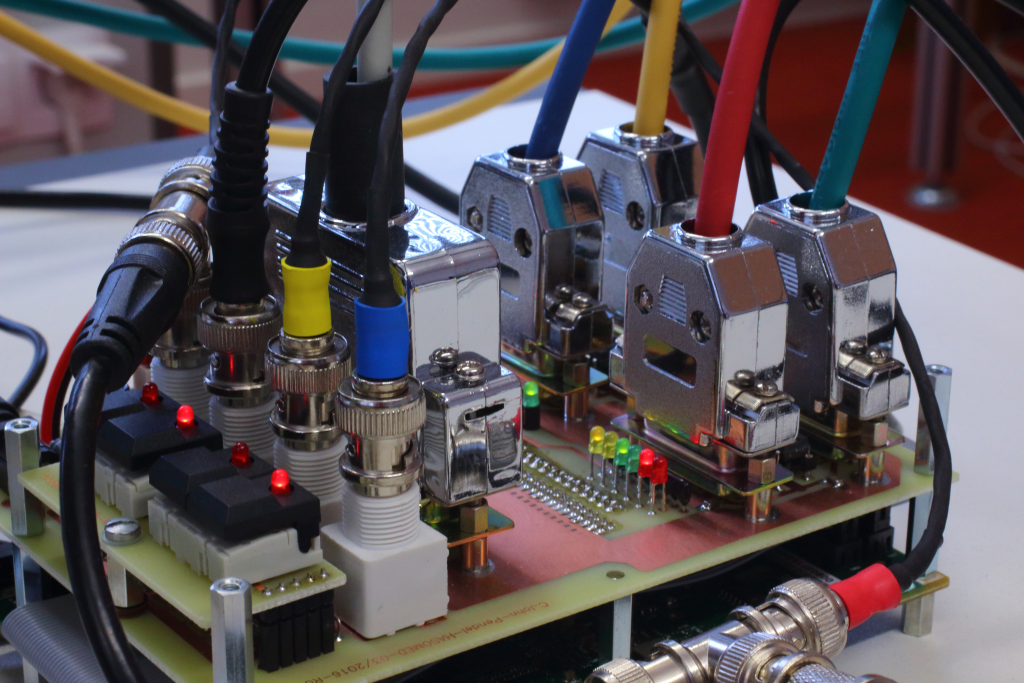
\includegraphics[width=0.7\textwidth]{bild}
\caption{Ein Hochleistungsschnittstellenboard wie es typisch in regelungstechnischen Echtzeitanwendungen ist, um höchsten technologischen Anforderungen im Rahmen der Industrie 4.0 gerecht zu werden.}
\label{fig:Bild}
\end{figure}


\subsection{Unter-unterabschnitt 1}

\blindmathtrue
\Blindtext[2][4]

\begin{figure}[ht]
\begin{subfigure}[c]{0.5\textwidth}
\centering
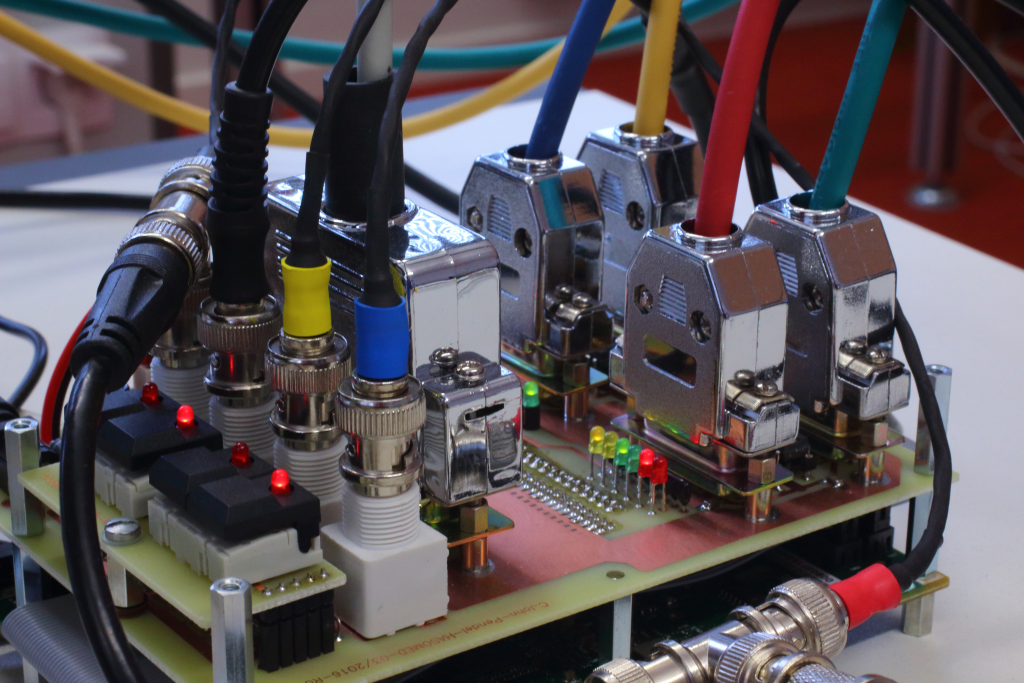
\includegraphics[width=0.7\textwidth]{bild}
\subcaption{Fall mit Synchronisation.}
\end{subfigure}
\begin{subfigure}[c]{0.5\textwidth}
\centering
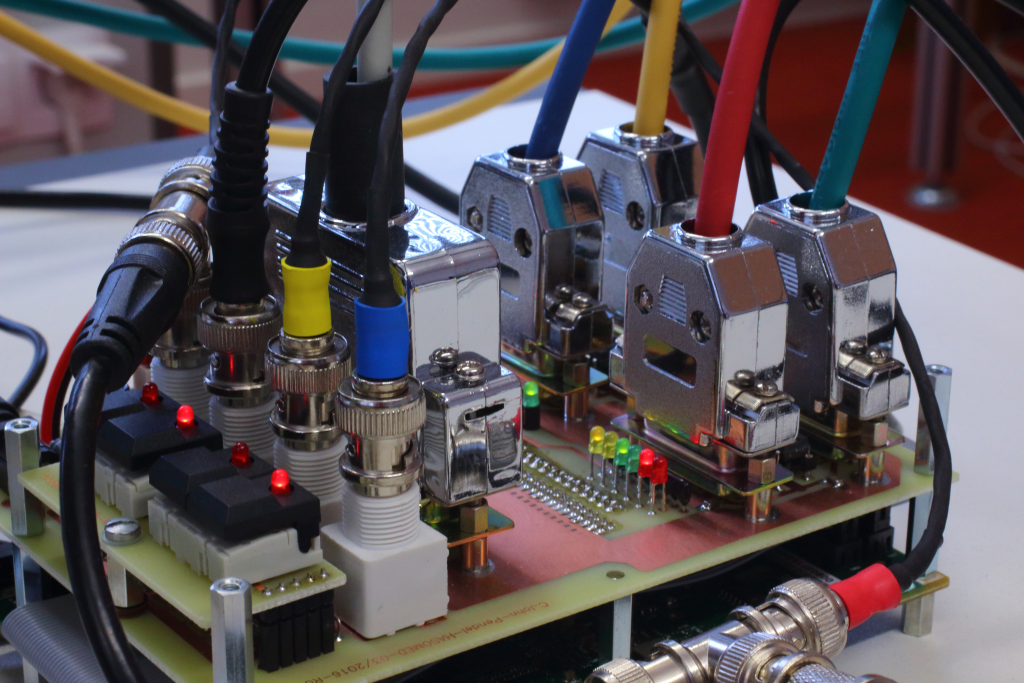
\includegraphics[width=0.7\textwidth]{bild}
\subcaption{Fall ohne Synchronisation.}
\end{subfigure}
\caption{Zwei verschiedene Anwendungsfälle für das Hochleistungsschnittstellenboard.}
\end{figure}










\subsection{Unter-unterabschnitt 2}

\blindmathfalse
\Blindtext[3][1]

\begin{figure}[ht]
\begin{subfigure}[c]{0.5\textwidth}
\centering
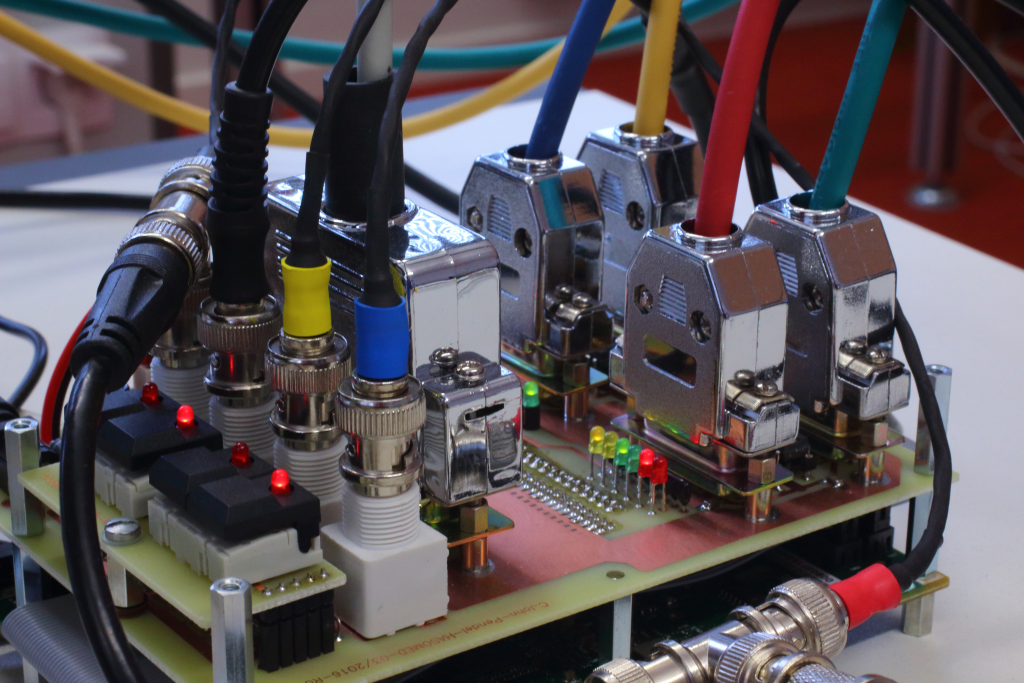
\includegraphics[width=0.7\textwidth]{bild}
\subcaption{Fall mit Synchronisation.}
\end{subfigure}
\begin{subfigure}[c]{0.5\textwidth}
\centering
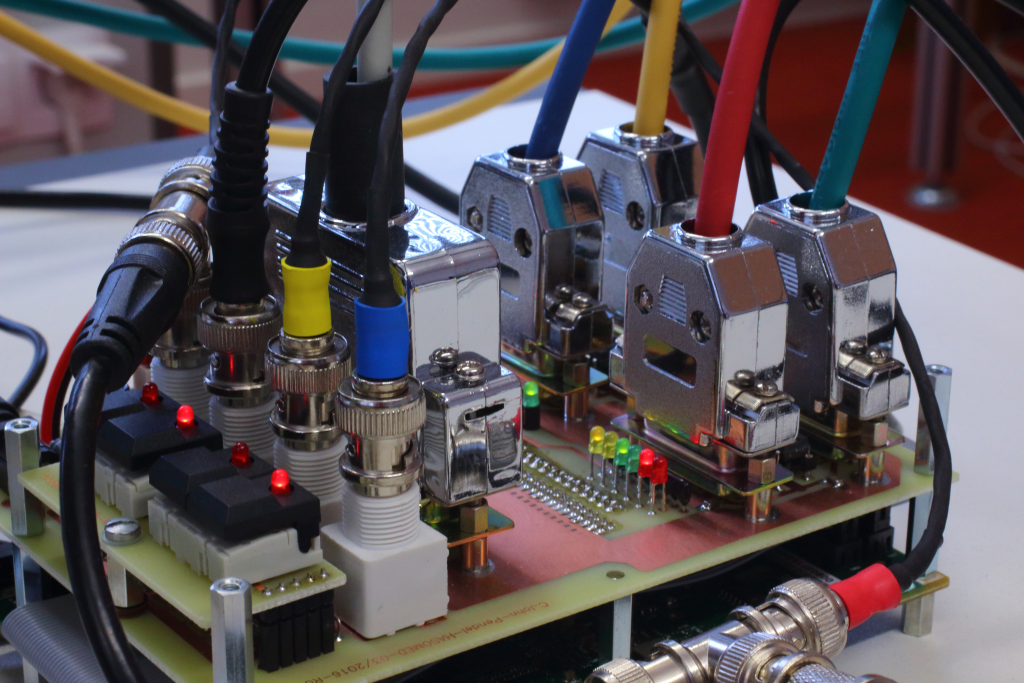
\includegraphics[width=0.7\textwidth]{bild}
\subcaption{Fall ohne Synchronisation.}
\end{subfigure}
\begin{subfigure}[c]{0.5\textwidth}
\centering
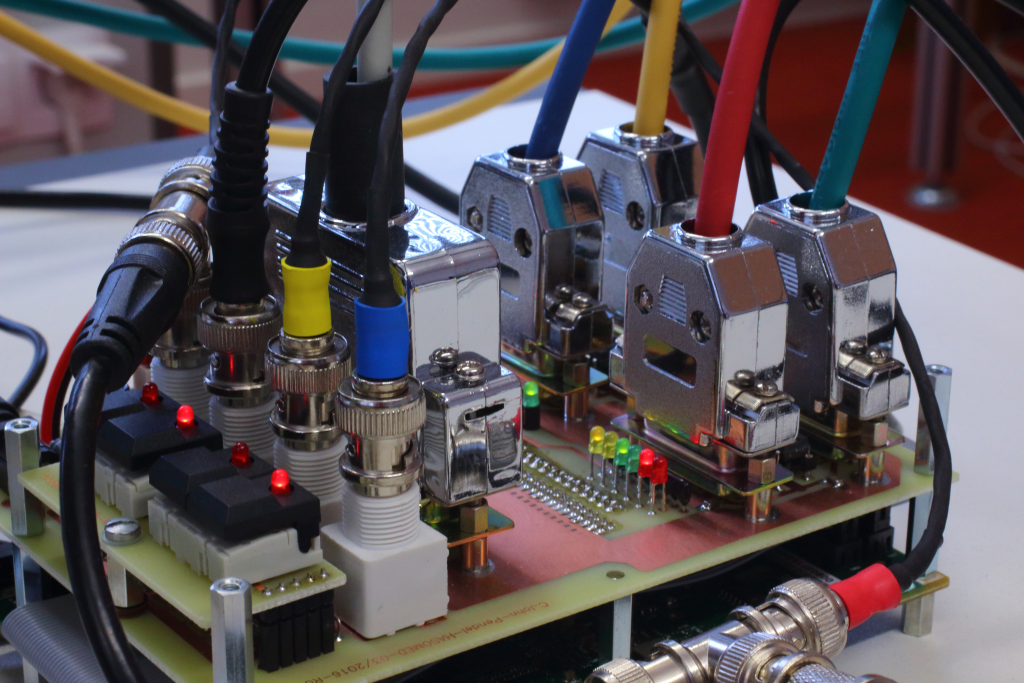
\includegraphics[width=0.7\textwidth]{bild}
\subcaption{Fall mit unterkritischer partieller Synchronisation.}
\end{subfigure}
\begin{subfigure}[c]{0.5\textwidth}
\centering
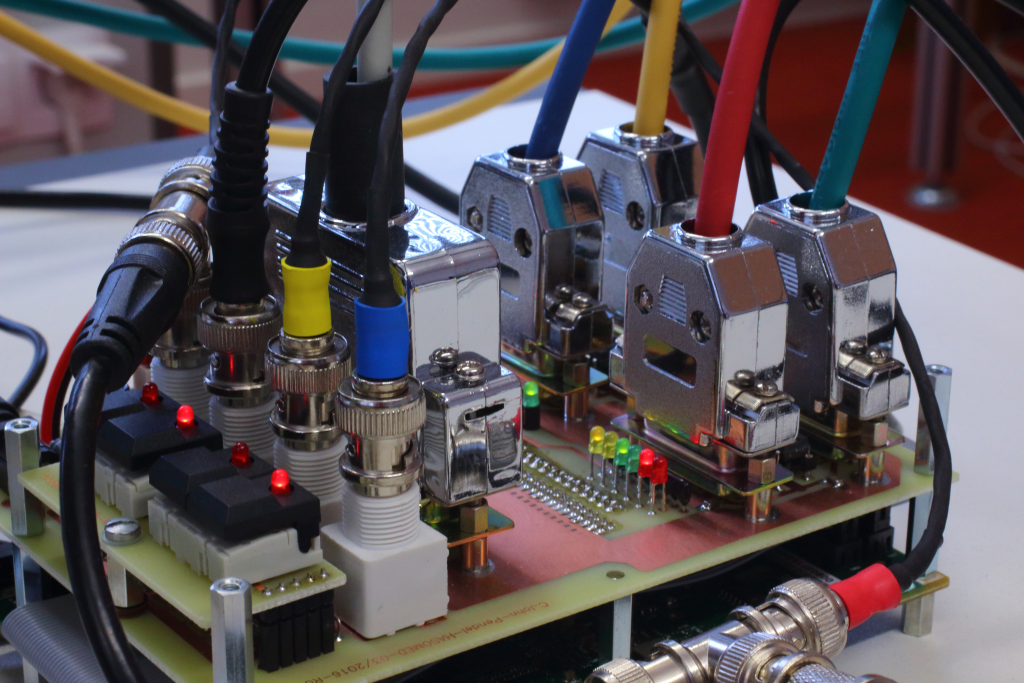
\includegraphics[width=0.7\textwidth]{bild}
\subcaption{Fall mit überkritischer partieller Synchronisation.}
\end{subfigure}
\caption{Vier verschiedene Anwendungsfälle für das Hochleistungsschnittstellenboard, die die unterschiedliche Leistungsfähigkeit demonstrieren.}
\end{figure}

\Blindtext[3][2]





% ==================================
% Literaturverzeichnis
% ==================================
\nocite{FLMR95ijc,Mik57de}

\bibliography{Arbeit}

\bibliographystyle{gerabbrv}
%\bibliographystyle{gerplain}

\end{document}


%%% Local Variables:
%%% mode: latex
%%% TeX-master: t
%%% End:
